\chapter{Tecnologias \textit{Web}}

\section{\textit{Framework}}
Segundo \citeonline{artigo_oo_reuso_software}, a programação orientada a objetos é muita vezes utilizada para promover o reuso de software. Para \citeonline{artigo_reuso_classes}, algumas linguagens, como \textit{Smalltalk}, são utilizadas tanto para reduzir o tempo de desenvolvimento quanto o custo de manutenções, simplificando a criação de novos sistemas e de novas versões para sistemas já existentes. Afirma, também, que “componentes de um programa devem ser projetados para reusabilidade”.

Novamente, segundo \citeonline{artigo_reuso_classes}, um “design abstrato orientado a objetos”, também chamado de \textit{framework}, consiste em uma interface para os principais componentes dentro de uma
arquitetura pré-definida. “\textit{Frameworks} proveem uma maneira de reutilizar código que é resistente a mais tentativas de reusos convencionais”, ou seja, componentes independentes de uma aplicação podem ser reutilizados mais facilmente.

\citeonline{artigo_reuso_classes}, compara “programas esqueletos” com \textit{frameworks}, os quais consistem em uma abordagem tradicional de reutilização de código e na garantia de consistência entre todos os componentes de um sistema sobre a mudança de algum requisito. O autor também realiza uma comparação entre os \textit{frameworks} do tipo “caixa-branca” e “caixa-preta”, onde o primeiro é responsável por especificar o comportamento de uma aplicação adicionando-se métodos para subclasses de uma ou mais de suas classes, ou seja, a implementação deste tipo de \textit{framework} deve ser conhecida para sua utilização, já o segundo consiste no uso de um protocolo responsável por definir uma interface entre os componentes, assim, o usuário precisaria entender apenas como funciona a interface externa dos componentes para utilizá-los.

\section{\textit{Django}}
O \textit{Django} é um \textit{framework} para desenvolvimento \textit{web} realizado na linguagem Python\footnote{\url{https://www.python.org/}}. Sua arquitetura baseia-se no modelo MTV (\textit{Model} \textit{Template} \textit{View}), onde:
\begin{itemize}
    \item \textit{Model}: representa as classes que popularão as tabelas do banco de dados. Além disso, utiliza os conceitos de ORM (\textit{Object-Relational Mapping}, Mapeamento de Objeto Relacional) para realizar a manipulação dessas tabelas, não sendo necessário a escrita de consultas em SQL para a persistência das informações.
    \item \textit{Template}: descreve como as informações serão apresentadas para o usuário.
    \item \textit{View}: representada por uma função \textit{callback} referente à uma respectiva URL, descrevendo quais informações serão apresentadas.
\end{itemize}

O Django utiliza aplicações dentro de um projeto, sendo estas responsáveis por uma funcionalidade específica do projeto. Cada aplicação possui suas próprias \textit{models}, \textit{views} e \textit{templates}.

A função de \textit{Controller} é realizado pela Django misturando as regras de negócio implementadas no modelo com os componentes do \textit{framework}, como o \textit{URL dispatcher} e os \textit{Middlewares}. O URL dispatcher identifica endereços requisitados pelo usuário e realiza o redirecionamento da requisição para a aplicação correta. Já os \textit{Middlewares} são componentes responsáveis pelo processamento de requisições e respostas.

A Figura \ref{django-arq} ilustra a arquitetura do \textit{Django}:

\begin{figure}[h]
    \centering
    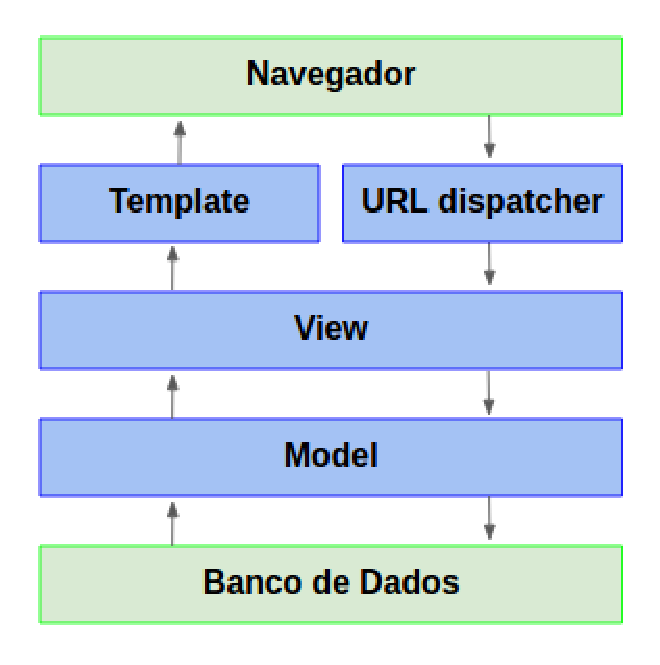
\includegraphics[keepaspectratio=true,scale=0.5]{figuras/django-arquitetura.eps}
    \caption{Arquitetura MTV \textit{Django}}
    \label{django-arq}
\end{figure}

\section{Ferramentas \textit{Web} Utilizadas}
    \subsection{\textit{Coverage}}
    Coverage\footnote{\url{https://pypi.python.org/pypi/coverage/}} é responsável por medir a cobertura de código utilizando ferramentas de análise e rastreando quais
    linhas de teste foram/devem ser executas.

    \subsection{\textit{GitLab CI}}
    \textit{GitLab CI}\footnote{\url{https://about.gitlab.com/gitlab-ci/}} baseia-se em uma ferramenta que oferece serviço de integração contínua ao projeto.

    \subsection{\textit{Matplotlib}}
    Matplotlib\footnote{\url{http://matplotlib.org/}} é uma biblioteca para produzir gráficos de alta qualidade em 2D/3D. Seus usos contemplam gráficos interativos, publicações científicas, interface de usuário e servidores de aplicativos \textit{web} para múltiplas interfaces de usuário.

    \subsection{\textit{Sphinx}}
    \textit{Sphinx}\footnote{\url{http://www.sphinx-doc.org/}} é uma ferramenta para criação inteligente e estilizada de documentação de códigos em \textit{python}, C/C++
    e outras linguagens. Utiliza \textit{reStructuredText} como sua linguagem de marcação e converte toda a documentação para formato html, pdf, epub ou man.

\section{Protocolos Utilizados}
    \subsection{\textit{Modbus RTU}}
    \textit{Modbus} é um protocolo serial utilizado para transmitir informações entre dispositivos eletrônicos. Suas mensagens utilizam os princípios de mestre-escravo, figura \ref{mestre_escravo}, onde o dispositivo requisitando a informação é chamado de mestre e os dispositivos fornecendo informações chamados de escravos. \cite{modbus}.
    \begin{figure}[!htpb]
        \centering
        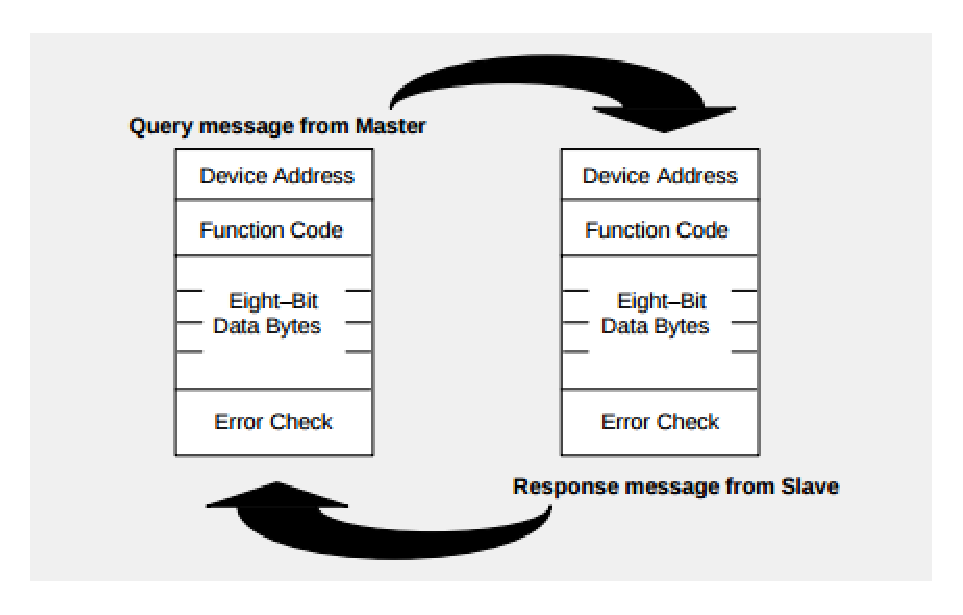
\includegraphics[keepaspectratio=true,scale=0.8]{figuras/mestre_escravo.eps}
        \caption{Comunicação Mestre-Escravo \textit{Modbus}. Fonte: \cite{modbus}}
        \label{mestre_escravo}
    \end{figure}

    Quando controladores são configurados para se comunicarem em uma rede Modbus usando o modo RTU (\textit{Remote Terminal Unit}, Unidade de Terminal Remoto) cada \textit{byte} contém duplas hexadecimais de 4 \textit{bits}. A maior vantagem de utilizar este modo é que sua grande densidade de caracteres permite uma maior taxa de transferência comparado ao modo ASCII, tendo a mesma taxa de transmissão \cite{modbus}.

    O cabeçalho de uma mensagem em Modbus RTU, figura \ref{modbusrtuheader}, possui 16 \textit{bytes} e é definido da seguinte maneira:
    \begin{itemize}
        \item Identificador do Aparelho: 2 \textit{bytes}.
        \item Código de Função: 2 \textit{bytes}, define qual tipo de operação o equipamento irá realizar.
        \item Campo de Dados: 8 \textit{bytes}, sendo 4 \textit{bytes} para indicar o endereço do primeiro registrador requisitado e 4 \textit{bytes} para indicar a quantidade de registradores que serão lidos.
        \item CRC (\textit{Cyclic Redundancy Check}, Verificação de Redundância Cíclica): 4 \textit{bytes} para verificação de erros.
    \end{itemize}

    \begin{figure}[!htpb]
        \centering
        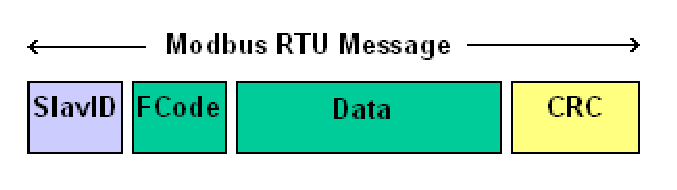
\includegraphics[keepaspectratio=true,scale=0.8]{figuras/modbusrtuheader.eps}
        \caption{Cabeçalho de uma Mensagem \textit{Modbus RTU}. Fonte: \cite{modbus_online}}
        \label{modbusrtuheader}
    \end{figure}

